\documentclass[12pt, a4paper]{article}
% Some fancy symbols
\usepackage{textcomp}
\usepackage{stmaryrd}
\usepackage{cancel}

% Some fancy symbols
\usepackage{textcomp}
\usepackage{stmaryrd}


\usepackage{array}

% Math packages
\usepackage{amsmath,amsthm,amssymb, amsfonts, mathrsfs, dsfont, mathtools}
% \usepackage{mathtext}

\usepackage[bb=boondox]{mathalfa}
\usepackage{bm}

% To conrol figures:
\usepackage{subfig}
\usepackage{adjustbox}
\usepackage{placeins}
\usepackage{rotating}



\usepackage{lipsum}
\usepackage{psvectorian} % Insanely fancy text separators!


% Refs:
\usepackage{url}
\usepackage[backref]{hyperref}

% Fancier tables and lists
\usepackage{booktabs}
\usepackage{enumitem}
% Don't indent paragraphs, leave some space between them
\usepackage{parskip}
% Hide page number when page is empty
\usepackage{emptypage}


\usepackage{multicol}
\usepackage{xcolor}

\usepackage[normalem]{ulem}

% For beautiful code listings:
% \usepackage{minted}
\usepackage{listings}

\usepackage{csquotes} % For citations
\usepackage[framemethod=tikz]{mdframed} % For further information see: http://marcodaniel.github.io/mdframed/

% Plots
\usepackage{pgfplots} 
\pgfplotsset{width=10cm,compat=1.9} 

% Fonts
\usepackage{unicode-math}
% \setmathfont{TeX Gyre Termes Math}

\usepackage{fontspec}
\usepackage{polyglossia}

% Named references to sections in document:
\usepackage{nameref}


% \setmainfont{Times New Roman}
\setdefaultlanguage{russian}

\newfontfamily\cyrillicfont{Kurale}
\setmainfont[Ligatures=TeX]{Kurale}
\setmonofont{Fira Code}

% Common number sets
\newcommand{\sN}{{\mathbb{N}}}
\newcommand{\sZ}{{\mathbb{Z}}}
\newcommand{\sZp}{{\mathbb{Z}^{+}}}
\newcommand{\sQ}{{\mathbb{Q}}}
\newcommand{\sR}{{\mathbb{R}}}
\newcommand{\sRp}{{\mathbb{R^{+}}}}
\newcommand{\sC}{{\mathbb{C}}}
\newcommand{\sB}{{\mathbb{B}}}

% Math operators

\makeatletter
\newcommand\RedeclareMathOperator{%
  \@ifstar{\def\rmo@s{m}\rmo@redeclare}{\def\rmo@s{o}\rmo@redeclare}%
}
% this is taken from \renew@command
\newcommand\rmo@redeclare[2]{%
  \begingroup \escapechar\m@ne\xdef\@gtempa{{\string#1}}\endgroup
  \expandafter\@ifundefined\@gtempa
     {\@latex@error{\noexpand#1undefined}\@ehc}%
     \relax
  \expandafter\rmo@declmathop\rmo@s{#1}{#2}}
% This is just \@declmathop without \@ifdefinable
\newcommand\rmo@declmathop[3]{%
  \DeclareRobustCommand{#2}{\qopname\newmcodes@#1{#3}}%
}
\@onlypreamble\RedeclareMathOperator
\makeatother


% Correction:
\definecolor{correct_color}{HTML}{009900}
\newcommand\correction[2]{\ensuremath{\:}{\color{red}{#1}}\ensuremath{\to }{\color{correct_color}{#2}}\ensuremath{\:}}
\newcommand\inGreen[1]{{\color{correct_color}{#1}}}

% Roman numbers && fancy symbs:
\newcommand{\RNumb}[1]{{\uppercase\expandafter{\romannumeral #1\relax}}}
\newcommand\textbb[1]{{$\mathbb{#1}$}}



% MD framed environments:
\mdfsetup{skipabove=1em,skipbelow=0em}

% \mdfdefinestyle{definition}{%
%     linewidth=2pt,%
%     frametitlebackgroundcolor=white,
%     % innertopmargin=\topskip,
% }

\theoremstyle{definition}
\newmdtheoremenv[nobreak=true]{definition}{Определение}
\newmdtheoremenv[nobreak=true]{theorem}{Теорема}
\newmdtheoremenv[nobreak=true]{lemma}{Лемма}
\newmdtheoremenv[nobreak=true]{problem}{Задача}
\newmdtheoremenv[nobreak=true]{property}{Свойство}
\newmdtheoremenv[nobreak=true]{statement}{Утверждение}
\newmdtheoremenv[nobreak=true]{corollary}{Следствие}
\newtheorem*{note}{Замечание}
\newtheorem*{example}{Пример}

% To mark logical parts
\newcommand{\existence}{{\circled{$\exists$}}}
\newcommand{\uniqueness}{{\circled{$\hspace{0.5px}!$}}}
\newcommand{\rightimp}{{\circled{$\Rightarrow$}}}
\newcommand{\leftimp}{{\circled{$\Leftarrow$}}}


% Useful symbols:
\renewcommand{\qed}{\ensuremath{\blacksquare}}
\renewcommand{\vec}[1]{\overrightarrow{#1}}
\newcommand{\eqdef}{\overset{\mathrm{def}}{=\joinrel=}}
\newcommand{\isdef}{\overset{\mathrm{def}}{\Longleftrightarrow}}
\newcommand{\inductdots}{\ensuremath{\overset{induction}{\cdots}}}

% Matrix's determinant
\newenvironment{detmatrix}
{
  \left|\begin{matrix}
}{
  \end{matrix}\right|
}

\newenvironment{complex}
{
  \left[\begin{gathered}
}{
  \end{gathered}\right.
}


\newcommand{\nl}{$~$\\}

\newcommand{\tit}{\maketitle\newpage}
\newcommand{\tittoc}{\tit\tableofcontents\newpage}


\newcommand{\vova}{  
    Латыпов Владимир (конспектор)\\
    {\small \texttt{t.me/donRumata03}, \texttt{github.com/donRumata03}, \texttt{donrumata03@gmail.com}}
}


\usepackage{tikz}
\newcommand{\circled}[1]{\tikz[baseline=(char.base)]{
            \node[shape=circle,draw,inner sep=2pt] (char) {#1};}}

\newcommand{\contradiction}{\circled{!!!}}

% Make especially big math:

\makeatletter
\newcommand{\biggg}{\bBigg@\thr@@}
\newcommand{\Biggg}{\bBigg@{4.5}}
\def\bigggl{\mathopen\biggg}
\def\bigggm{\mathrel\biggg}
\def\bigggr{\mathclose\biggg}
\def\Bigggl{\mathopen\Biggg}
\def\Bigggm{\mathrel\Biggg}
\def\Bigggr{\mathclose\Biggg}
\makeatother


% Texts dividers:

\newcommand{\ornamentleft}{%
    \psvectorian[width=2em]{2}%
}
\newcommand{\ornamentright}{%
    \psvectorian[width=2em,mirror]{2}%
}
\newcommand{\ornamentbreak}{%
    \begin{center}
    \ornamentleft\quad\ornamentright
    \end{center}%
}
\newcommand{\ornamentheader}[1]{%
    \begin{center}
    \ornamentleft
    \quad{\large\emph{#1}}\quad % style as desired
    \ornamentright
    \end{center}%
}


% Math operators

\DeclareMathOperator{\sgn}{sgn}
\DeclareMathOperator{\id}{id}
\DeclareMathOperator{\rg}{rg}
\DeclareMathOperator{\determinant}{det}

\DeclareMathOperator{\Aut}{Aut}

\DeclareMathOperator{\Sim}{Sim}
\DeclareMathOperator{\Alt}{Alt}



\DeclareMathOperator{\Int}{Int}
\DeclareMathOperator{\Cl}{Cl}
\DeclareMathOperator{\Ext}{Ext}
\DeclareMathOperator{\Fr}{Fr}


\RedeclareMathOperator{\Re}{Re}
\RedeclareMathOperator{\Im}{Im}


\DeclareMathOperator{\Img}{Im}
\DeclareMathOperator{\Ker}{Ker}
\DeclareMathOperator{\Lin}{Lin}
\DeclareMathOperator{\Span}{span}

\DeclareMathOperator{\tr}{tr}
\DeclareMathOperator{\conj}{conj}
\DeclareMathOperator{\diag}{diag}

\expandafter\let\expandafter\originald\csname\encodingdefault\string\d\endcsname
\DeclareRobustCommand*\d
  {\ifmmode\mathop{}\!\mathrm{d}\else\expandafter\originald\fi}

\newcommand\restr[2]{{% we make the whole thing an ordinary symbol
  \left.\kern-\nulldelimiterspace % automatically resize the bar with \right
  #1 % the function
  \vphantom{\big|} % pretend it's a little taller at normal size
  \right|_{#2} % this is the delimiter
  }}

\newcommand{\splitdoc}{\noindent\makebox[\linewidth]{\rule{\paperwidth}{0.4pt}}}

% \newcommand{\hm}[1]{#1\nobreak\discretionary{}{\hbox{\ensuremath{#1}}}{}}


\renewcommand{\labelenumii}{\theenumii}
\renewcommand{\theenumii}{\theenumi.\arabic{enumii}.}

\graphicspath{{images/}}


\title{Конспект к экзамену по билетам (архаичные ЭВМ) \\ 1-й семестр} 

\author{
  \vova
  \and
  Скаков Павел Сергеевич (лектор)\\
  \texttt{t.me/pavelxs}
}

\date{\today}



\begin{document}

\maketitle
\newpage
\tableofcontents
\newpage


\section{Введение}

Максимально сжатый материал: если читатель не знаком с курсом, возможно, 
стоит сначала изучить конспект Тимофея на Overleaf.


\section{Названия билетов (ровно как в оригинале)}

\begin{enumerate}
    \item Устройство памяти
    \begin{enumerate}
        \item Элементная база вычислительной системы: логические элементы, триггеры.
        \item Оперативная память: статическая/динамическая, организация.
        \item Оперативная память: характеристики, типы динамической памяти. NUMA.
        \item Кэш-память.
        \item Протоколы когерентности кэш-памяти.
        \item Носители информации: магнитные, оптические и на основе флеш-памяти. RAID.
    \end{enumerate}
    
    
    \item Архитектура процессорных систем
    \begin{enumerate}
        \item Архитектура фон Неймана и её альтернативы.
        \item Архитектура набора команд (ISA) и микроархитектура.
        \item Конвейерная архитектура. Конвейер MIPS.
        \item Проблемы конвейера (hazards) и пути их решения.
        \item Суперскалярная и VLIW архитектуры. Спекулятивное исполнение. Уязвимости классов Spectre и Meltdown.
        \item Многоядерные/многопроцессорные системы, одновременная многопоточность (SMT/HT).
    \end{enumerate}
\end{enumerate}

Нужно ответить на два вопроса: по одному из каждой части. Пользоваться ничем нельзя, отвечать сразу.


\section{Устройство памяти: О чём говорить при каждом из билетов?}


\subsection{Элементная база вычислительной системы: логические элементы, триггеры.}

Европейские и американские обозначения логических элементов

Полусумматоры и сумматоры (медиана + $XOR$ или два полусумматора + $OR$)

RS-триггер, каноническая и енаиболее эффективная версия — через два ИЛИ-НЕ.

Проблемы высоких частот и малого размера, «В Ethernet соотношение сигнал/шум — как разговаривать рядом с турбиной самолёта»

$\Longrightarrow$ Синхронная версия RS-триггера, D-триггер через «не» на входе.



\subsubsection{MEM}

Декодер 3to8 (для каждого из 8 выходов $AND$ от трёх, возможно, инвертированных входов) 
$\Longrightarrow$ мультиплексор ($3 + 8 → 1$) и демультиплексор ($3 + 1 → 8$).

Из этого можно сделать модуль памяти «Mem» на 8 бит: 

Входы: 3 адресных бита, $R/W$, $C$ (clock), $D$ (запись, если выбран режим $W$).

Выход: «Q» — если выбран режим $R$ (не обязательно только в этому случае)
— на нём значение, соответствующее биту по адресу $\overline{A_0 \! A_1 \! A_2}$.


\subsubsection{JK-триггер}

JK-триггер (Входы $J, K$, синхронный, $\Lleftarrow$ умеет инвертировать состояние при двух единицах). 
Крафтится из двух RS-триггеров с тактированием в противофазе, 
на вход первого кроме оригинальных входов $J, K$ через «AND» даётся то, 
что запомнил второй (то есть что было на первом до начала такта).
В нормальной версии результат ($Q$ и $\tilde Q$) берётся из выходов первого триггера.

\subsubsection{Физические основы работы логических элементов}

Нас интересуют в основном транзисторы.

Транзистор: затвор влияет на электрические характеристики перехода исток-сток.
Биполярный: влияет \textbf{ток} через затвор (на самом деле, называется «база»)
Полярный: влияет \textbf{напряжение} на затворе

n-канальные полярные транзисторы. Исток — «внизу», то есть там напряжение ниже, чем на стоке. Состоит из 

Напряжение считаем относительно истока. 
Подложку мы заземляем, чтобы не влияла на электрическое поле, которое создается остальными элементами.
Если подать положительно напряжение на затвор (опять же, относительно истока), а в случае p-типа — отрицательное, 
притянутся электроны и образуется насыщенный электронами канал между двумя проводниками.

\subsubsection{Логики}

По многим причинам победила $CMOS$-логика, конструирующая только транзисторы (причём полевые)
для конструкции элементов. Это позволяет минимизировать потребляемую энергию, так как ток течёт только при переключении.
В отличие от полевых транзисторов (где он нужен через базу для поддержания открытого состояния),
а также $NMOS$ логики, где он течёт по резистору в некоторых случаях (когда транзистор открыт).

В случае $CMOS$ логики расход энергии растёт при увеличении частоты почти линейно по понятным причинам.

\begin{figure}[h!]
    \centering
    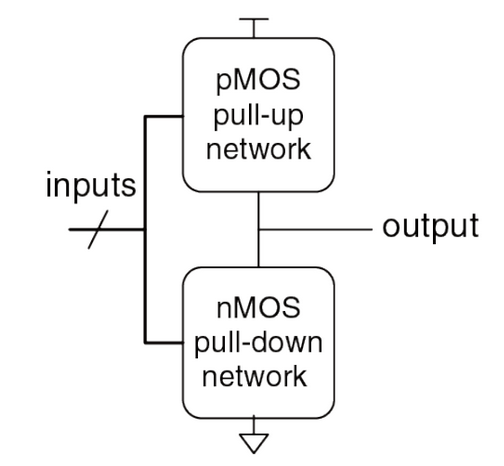
\includegraphics[width=\textwidth]{images/general_cmos_element_scheme.png}
    \caption{Общий принцип построения схем в CMOS логике}
    \label{fig:cmos_general}
\end{figure}
\FloatBarrier

В качестве элементарных частиц используем $NOT, NAND, NOR$ (нельзя сделать $AND$ и $OR$ эффективнее, чем соответствующий $NAND/NOR \circ NOT$)

Fun Fact: можно сделать $NOR$ и $NAND$ на много входов эффективнее, чем просто внешне композировать (например, для трёх — 6 вместо 8-и).


\subsubsection{Дребезг контактов}

Кнопки из реальной жизни при нажатии не сразу устанавливается в новой состояние, а сначала колеблется. 
Это назвается Contact bounce (дребезг контактов). Причём чем старше и некачественнее контакты, тем дольше будет происходить bouncing.

Есть несколько подходов к борьбе с ним. Бывает, программно, бывает аппаратно.
Причём криме вопросов реализации возникают ещё и концептуальные. 
Проще всего реагировать на нажатие с запозданием: по истечении времени с начала или с последнего изменения.
Другой вариант — реагировать как только произошло изменение после затишья, но после этого игнорировать дребезг, пока не установится.
Однако, если у нас не просто бинарная кнопка с одним контактом «нажат/не нажат», 
а имеющая положения «не нажата, положение 1 и положение 2» и мы хотим на выход подавать бинарный сигнал в виде последнего «ка\'санного» контакта, 
то всё гораздо очевиднее и у нас есть ультимативное решение через триггер и, возможно, транзистор.
Не забыть про подтягивающие резисторы.




\subsection{Оперативная память: статическая/динамическая, организация.}

Папмять располагают в 2D решётчатой структуре.

Количество проводов $\propto cols + rows  \Rightarrow O(\sqrt{memory\_size})$

$Row$ отвечает за выбор ряда. Если он ноль, ячейка вообще не работает.

Если подаётся $true$, ячейка открывается. Можно считывать информацию с соответствующих $Col$ и $\overline{Col}$.
Также можно записывать на эти входы.


Статическая память строится как 

\begin{center}
    \begin{tabular}{|| m{10em} | m{10em} | m{12em} ||} 
     \hline
     &                          \textbf{Статическая память}  & \textbf{Динамическая память} \\ [0.5ex] 
     \hline\hline
     Скорость &                 быстрая             & медленная \\ 
     \hline 
     Количество транзисторов &  Много (≈6)          & Мало (обычно один + кондерсатор) \\ 
     \hline
     Надёжность &  Наличествует          & Постоянно дегенерирует $\Rightarrow$ надо регенерировать  \\
     \hline
     Примеры &  Регистры, кэш          & Оперативная память, видеопамять  \\
     \hline
    \end{tabular}
\end{center}

Параметры, по которым оценивается память:
\begin{center}
    Объём, 
    
    скорость доступа («latency»), 
    
    скорость передачи («throughput», пропускная способность)
\end{center}

Уязвимость Raw-Hammer: если очень долго обращаться к ячейкам, соседним с данной, можно установить её в ноль.




\subsection{Оперативная память: характеристики, типы динамической памяти. NUMA.}

Адресуемся в порядке: старшие биты адреса — номер строки, младшие — номер столбца.

Типичные интерфейсные выводы оперативки:

\begin{itemize}
    \item 
\end{itemize}

Порядок работы с памятью: 
\begin{enumerate}
    \item Процессор сообщает о таймингах
    \item Всё время идет синхронизация 
    \item Выбор строки $\Rightarrow$ модуль динамической памяти заносит строку в статическую
    \item Работа со строкой: запрос адреса
    \item После передачи данных и выбора следующей строки происходит «закрытие» старой 
    — в динамические ячейки вновь записываются данные из статической строки.
    \item 
\end{enumerate}

Что какие тайминги означают?

Аббривеатуры: 
\begin{itemize}
    \item $RAS$ — Row Access Strobe — сигнал выборки строки
    \item $CAS$ — Column Access Strobe — $—"—$ столбца
    \item Precharge — «закрытие строчки»
\end{itemize}

\begin{itemize}
    \item $CL$ — CAS Latency — с получения адреса столбца до ответа
    \item $t_{RCD}$ — RAS to CAS Delay — открытие строки
    \item $t_{RP}$ — Row Precharge — закрытие строки
    \item $t_{RAS}$ — Минимальное время активности строки
\end{itemize}


Производители обычно указывают либо 4 тайминга:

\begin{equation*}
    CL - t_{RCD} - t_{RP} - t_{RAS}
\end{equation*}

Либо только $CL$.

Причём измеряется это в количестве тактов при какой-то заданной частоте.

Если обращаемся к памяти редко, задержка будет $t_{RCD} + t_{CL}$.
Если часто, причём в случайные строки, то $t_{RAS} + t_{RP}$

Улучшенные стандарты памяти: 
\begin{itemize}
    \item FPM DRAM: можно работать с одной строкой сколько угодно, не закрывая её
    \item EDO RAM: можно держать столбец не до самого конца чтения, а отпускать, пока ждём CL
    \item BEDO DRAM: выдаёт вместе с ячейкой памяти выдаётся 3 следующих (если кончается на $…00$)
    \item SDRAM: модуль и контроллер памяти работают синхронно + за один запрос отправляем не 32 бита, а 64
    \item DDR SDRAM: передаём данные по двум тактовым сигналам в противофазе (и по восходящему фронту, и по нисходящему)
    \item DDR2 SDRAM: увеличили тактовую частоту в 2 раза, а внутри стала больше только передающая шина
    \item DDR3 SDRAM: Ещё в 2 раза. Итого — 512 бит
    \item DDR4 SDRAM: мелкие технические улучшения
\end{itemize}

GDDR: максимизируем скорость передачи, на доступ забиваем


Существуют двух- и более портовые ячейки памяти. Есть тот же бит, но много интерфейсных транзисторов.
На каждый — новые «$Col_k$», «$Row_k$»

На практике используется редко, так как сложно изготавливать. 

\textbf{Многобанковая vs. Многоранговая vs. Многоканальная памяти.}

Многобанковая: одному модулю памяти соответствует несколько банок — матриц
Многоранговая: в одном физическом блоке (слоте) есть несколько модулей
Многоканальная: параллельные слоты под память, для $fine-grained$ параллелизма нужны похожие модули.


\subsection{Кэш-память.}

Это такой большой костыль, возникший из-за того, что процессоры стали быстрее памяти.
Находится близко к вычислительным ядрам, на кристале процессора.
Делает то, о чём говорит его название: кэширует запросы к памяти.
Имеет меньший размер, чем оперативка, но работает быстрее.

Работа основана на идеи адресно-временной локальности.

«look aside» vs. «look through»

«write through» vs. «write back»


\subsection{Протоколы когерентности кэш-памяти.}

Зачем нужно поддержание когерентности? (пример с DeadLock-ом из-за отсутствия когерентности).
Можно решать на уровне пргограммиста, можно — на уровне железа. 
Второе лучше, так как может учитывать контекст исполнения. 
То есть сбрасывать кэш может быть не нужно, если, например, он сейчас только у этого ядра.


Обозначения сигналов:

\begin{itemize}
    \item \textcolor{red}{PR} — это ядро изволиои хотеть читать
    \item \textcolor{red}{PW} — это ядро изволиои хотеть писать
    \item \textcolor{green}{BR} — этот кэш отправляет по шине запрос на чтение
    \item \textcolor{green}{BRfO} — этот кэш отправляет по шине запрос на чтение + получение Ownership
    \item \textcolor{green}{BU} — этот кэш уже имеет данные, но хочет стать единственным владельцем, говорит другим «кыш»
    \item \textcolor{blue}{BR} — этот кэш получает по шине от другого кэша запрос на чтение
    \item \textcolor{blue}{BRfO} — этот кэш получает по шине от другого кэша запрос + получение Ownership
    \item \textcolor{blue}{BU} — \textbf{другой} кэш уже имеет данные, но хочет стать единственным владельцем, говорит другим «кыш»
    \item \textcolor{green}{Data} — ответ данными
    \item \textcolor{green}{DataW} — ответ данными + запись в оперативку
\end{itemize}

$MSI$:

\begin{itemize}
    \item $M$ — Modified — уникальное изменённое состояние кэш-линии
    \item $S$ — Shared — точная закэшированная копия оперативки
    \item $I$ — Invalid — данная кэш-линия отсутствует в кэше.
\end{itemize}

Важно, что из кэша могут выселять, тогда при $M$ мы записываем в память.

$MESI$ — решает проблему, что при любом \textcolor{red}{PW} из состояния $S$ отправляем всем сигнал \textcolor{green}{BU}.
Это забивает шину, хотя большая часть данных используется только в одном ядре.

Добавляется состояние $E$ — «exclusive» — уникальная, но всё ещё копия оперативной памяти.

Тут становится важно, кто отвечает на запрос о $BR$. Если память, переходим в $E$, иначе — в $S$.
И отвечать на запрос, конечно, становится обязательным.

$MESIF$. Добавляется состояние $F$ — Forwarded. Передаётся как эстафета, живёт у последнего прочитавшего Shared.
Если кто-то выкинул, то новым прижётся идти в оперативную память.


Другой вариант — $MOESI$. Состояние $O$ — Owner — появляется, если кто-то хочет прочитать данные, а они Modified.

Раньше в $Intel$ был $MESIF$, в AMD — $MOESI$, теперь — неизвестно.

\subsection{Носители информации: магнитные, оптические и на основе флеш-памяти. RAID.}

Дискреты

Cylinder-Head-Sector

В каждом секторе ≈512 байт. В каждом хранится адрес, CRC, а потом ещё ECC поверх всего.

HDD

LDA — Logical block adressing (теперь количество секторов уменьшают ближе к центру => адресацией занимается кто-то другой)

Эффективнее делать секторы побольше (сейчас — 4кБ), чтобы качественнее исправлять, но так как все захардкодили 512, 
диски притворяются, что у них столько и есть. Но если нужно весь сектор, плохо, так как читаем его 8 раз.

SMART — Self Monitoring And Reporting System

Shingled-винчестеры

Оптичекие диски

Секторы расположены в форме спирали, информация — есть дырка или нет, делать и проверять их наличие может лазер.

Бывает несколько слоёв: фокусировка лазера.

Audio CD: не нужны CRC и ECC.




и плёнки.

Флеш-память: используются тарнзисторы с плавающим затвором, в которые можно заселять или выселять электроны.

RAID — комбинация дисков для увеличения скорости и/или отказоустойчивости.


\section{Архитектура процессорных систем: О чём говорить при каждом из билетов?}

\subsection{Архитектура фон Неймана и её альтернативы.}

\begin{enumerate}
    \item Двоичная система счисления (главное — не 10-ная)
    \item Наличие чётких (абсолбтных и постоянных) адресов (vs. Машина Тьюринга)
    \item Последовательное выполнение инстукций (vs. Конвейер)
    \item Общая память для инструкций и данных (vs. Гарвардская)
\end{enumerate}



\subsection{Архитектура набора команд (ISA) и микроархитектура.}

Стековая, кумулятивная, Reg-Reg, Reg-Mem.




\section{Appendix}

\subsection{Получение каждого хазарда}

\subsection{Data хазарды}

Вознкают, если новые блихко расположенные инструкции зависимы от результатов предыдущих.

\subsubsection{RaW Data}

Сначала какая-то инструкция пишет, потому другая должна прочитать, что она записала, но читает старые данные $\Rightarrow$ hazard.

Пример: из $MIPS$.



\subsubsection{WaR Data}

Сначала какая-то инструкция читает, потому другая должна записать, но записывает раньше и первая читает новые данные вместо старых $\Rightarrow$ hazard.

Пример: из SuperScalar (OoO/OoO).

DIV R1, R2, R3

ADD R4, R1, R5

SUB R5, R6, R7

Если SS исполнит SUB раньше DIV (оно ведь от него не зависит?!), а это сделать хочется, так как умный конвейер занят,
то ADD считает новые данные вместо старых, так как выполнится после DIV, то есть и после SUB.

Одно из решений — аппаратно изменять соответствие между пользовательскими регистрами ($R_i$) 
и аппаратными.


\subsubsection{WaW Data}

Запись данных происходит не в том порядке, в результате оказывается не то значение.

Пример: из SuperScalar.
Берём наивный InO/OoO.

Div R1, R2, R3

Add R1, R4, R5



\subsubsection{Control}

Возникает из-за инструкций передачи контроля.
Если выполнять $JMP$ на $EX$, то на конвейер зайдёт ещё две команды, что плохо.
На $MIPS$ решают переносом его в $ID$ + докуменацией, что есть Delay Slot.


\subsubsection{Struct}

Не хватает скорости памяти. Одновременно к ней обращаются IF и MEM.
Побеждает MEM. 

Решения: либо успользовать гарвардскую архитектуру, либо ускорять память, либо по конвейеру отправляются NOP-ы.



\end{document}